\chapter{Sistema Interpretador de Faturas} 
\label{c:sistema_interpretador_de_faturas}
% ---
Descrita a parte de obtenção dos dados dos medidores, uma outra importante fonte de dados, principalmente econômicos, são as faturas de energia, porém devido ao grande número de unidades consumidoras da UFG essa análise e obtenção dos dados apenas de maneira manual seria algo com um alto custo, por isso, foi desenvolvido um sistema capaz de fazer uma carga em massa das faturas, que fosse capaz de interpretar os dados e gerar um resultado para análise tanto por softwares de \textit{business intelligence} tanto como poder alimentar o banco de dados do SIDE.

Este sistema pode ser executado independente do sistema operacional por se tratar de uma aplicação java, que é multiplataforma, e de maneira independente do banco de dados, sendo capaz de gerar um arquivo CSV com os dados extraídos das faturas contidas em um diretório selecionado e seus sub-diretórios, além de ser possível a alimentação do banco quando o dispositivo no qual for executado, tiver acesso a rede e os dados de acesso ao banco de dados do SIDE. Abaixo segue uma captura da tela do sistema \textit{PdfReader}:

\begin{figure}[H]
    \centering
    \caption{Tela Principal do Sistema PdfReader}
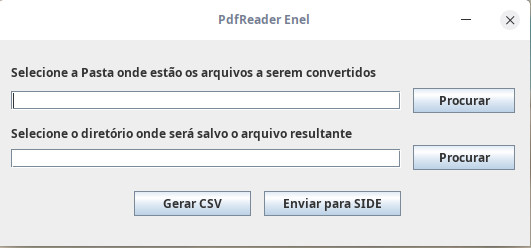
\includegraphics[width=\linewidth]{imagens/pdf-reader.png}
    \caption*{Fonte: Próprio Autor}
    \label{fig:diagrama-modelo-dados}
\end{figure}

\newpage
\section{Processo de Interpretação da Fatura}

Após selecionado o diretório de origem e o de destino do arquivo resultante, ao clicar em um dos dois botões de ação é executado o seguinte código abaixo:

\begin{listing}[ht]

\label{listing:sidesynchronizer}
\caption{Código Principal \textit{PdfReader}}
\inputminted[frame=lines,
    firstline=26,
    lastline=52,
    framesep=5mm, fontsize=\footnotesize, linenos=true, label={App.java}]{java}{codigos/PdfReader/App.java}
\end{listing}

Inicialmente é criado um arquivo temporário para armazenamento das conversões de pdf para texto puro das faturas, após é inicializado uma \textit{Collection} com todos os arquivos dentro do diretório passado como parâmetro através da variável \textit{path}, e esses arquivos são iterados fazendo inicialmente em cada arquivo a validação se o mesmo é um arquivo com a extensão PDF após isso é feita interpretação da primeira página da fatura onde, dependendo da opção selecionada será carregado o CSV ou o banco com esses dados coletados.

Após a leitura da primeira página o mesmo processo ocorre para a segunda página, e assim sucessivamente até todos os arquivos terem sido lidos, retornando para a tela principal com a mensagem de leitura efetivada com sucesso.r